% Here the formulas and description of what we used theoretically
%\documentclass{article}
%\begin{document}
\label{proposed}
\subsection{Networks}\label{proposed_networks}
Three network models of particular relevance for this project are the small-world model \cite{watts1998collective} from Watts and Strogatz and the Erd\"{o}s-R\'{e}nyi model for random networks \cite{erdos1960evolution} and regular ring latices. Small-world networks inhabit the space between the regular networks or lattices and random networks. Many practical networks have been shown to have a small-world topology, such as the nternet, the power grid amd neural networks,  for some more examples see \cite{albert2002statistical}. Small world-networks have a high cluster coefficient and low characteristic path length, means that  whereas random networks have a low characteristic path and low cluster coefficient and lattices have high cluster coefficients but long characteristic path length.

Coloquially explained in terms of my social network, a large(close to 1 ) cluster coefficient means that many of my friends know each other. A low characteristic path length means that I am connected to anyone on the world through small friends-of-friends chains.

Formally, let $G=(V, E)$ be a graph, where $V$ is a set of vertices, and $E$ a set of edges between vertices in $V$, here $e_{ij}$ denotes the edge connecting $i$ and $j$.  The \textit{out-neighborhood} of $v_i$, $N_i^{out}:=\{v_j|e_{ij}\in E\}$, the \textit{in-neighborhood} $N_i^{in}:=\{v_j|e_{ji}\in E\}$. The \textit{neighborhood} of $v_i$, $N_i:=N_i^{out}\cup N_i^{in}$. The \textit{degree} of vertex $v_i$, $k_i:=|N_i|$ is the number of vertices in the neighborhood of $v_i$, this can similarly be defined for in and out neigborhoods. The directional clustering coefficient for $v_i$ with $k_i>1$ can now be defined as:
$$C_i :=\frac{|\{e_{jk}\}|}{k_i(k_i-1)},$$
where $v_j,v_k\in N_i$ and $e_{jk}\in E$, let $n=|V|$ denote the number vertices the \textit{directional clustering coefficient} for $G$ is defined as:
$$C_G:=\frac{\sum_{i\in V} C_i}{n}.$$
The \textit{characteristic path length} $L_G$ of graph $G$ is the average shortest path length between vertices in $G$. Land  $L_{Gij}$ denote the length of the shortest path between vertices $i$ and $j$. 
$$L_G:= \frac{\sum_{i\in V} \sum_{j \in V\setminus i}L_{Gij}}{n(n-1)}.$$ 
Note finding all shortest paths can be performed using the Floyd-Warshall algorithm which has $O(|V|^3)$ complexity\cite{Floyd}.

For networks where $n\gg k\gg ln(n) \gg1$, the ring lattice will have $L_{lattice}\approx\frac{n}{2k}$ and $C_{lattice}\approx\frac{3}{4}$.
A large random network  $ L_{random}\approx\frac{\ln(n)}{\ln(k)}$ and $C_{random}=\frac{k}{n}$. A network is considered small world when $L_G\approx L_{random}$ and $C_G \gg C_{random}$

To find the core of most connected vertices we use the corefind algorithm, showin in Algorithm \ref{alg:findcore}.This algorithm recursively removes all vertices of degree $x$ from the network, starting at $1$. If there are vertices left in the network we repeat this with $x+1$. Once an empty network is obtained the previous network is deemed the core, because recursively removing nodes of heigher degree will inevitably lead to an empty network. The choice of the $degree(j)$ - standard, in-degree, out-degree,  or in+out-degree - facilitates in finding cores with different characteristics.

%\algsetup{indent=2em}
%\newcommand{\FindCore}{\ensuremath{\mbox{\sc FindCore}}}
%\begin{algorithm}[h!]
%\caption{$\FindCore(Network)$}\label{alg:findcore}
%\begin{algorithmic}
%\REQUIRE A Network $G=(V,E)$.
%\ENSURE The Core of Network $G$ and the degree $x$ at which the core is found.
%\medskip
%\STATE $x\gets 1$
%\WHILE {$|V| > 0$}
%	
%	\STATE $Gprevious \gets G$
%	\WHILE {$|\{j\in V | degree(j)<x\}| > 0$}
%		\STATE $G\gets removeNodes(G, \{j\in V | degree(j)<x\})$ 
%	\ENDWHILE
%	\STATE $i \gets x+1$
%\ENDWHILE
%\RETURN $Gprevious, x-1$
%\end{algorithmic}
%\end{algorithm}


\subsection{Feature extraction}
\label{sec:features}
When working with images, it is usually not possible to work with the raw image data (the pixel values). The reason for this is the high dimensionality of images, which can easily exist in a space of more than a million dimensions. By extracting features from images, they can be represented in a lower dimensional feature-space.  This feature extraction process has several advantages:
\begin{itemize}
\item The data becomes computationally easier to work with due to the smaller number of dimensions
\item By using the right features, the data becomes more suitable for generalization across images
\item Reducing the dimensionality makes it easier to visualize sets of images
\item Features can have an intuitive basis, which makes it easier for non-computer-scientists to analyze (sets of) images
\end{itemize}

% Computer vision is an important and maturing engineering science. It underpins an increasing variety of applications that require the acquisition, analysis, and interpretation of visual information.
In the extraction of image features, a distinction was made between low-level statistical features and higher level cognitive-based features....

\subsubsection{Statistical features}
As statistical features, many relatively simple low-level features were extracted from the images.
The first type of statistical features that were used are color-based features, which should capture the color-usage in the artwork. Many artists produce collections of art pieces with similar colors, and should therefore be (partially) distinguishable with color-based features. For each of the three RGB channels, an average and median is calculated over all the channel values. Let $\{\mathbf{x}_{m,i,c} \}_{i=1\dots n}$ be the pixel values for image $m$ in color channel $c \in \{R,G,B \}$. The average in channel $c$ of image $m$ is then given by 

\begin{equation}
\label{avgChannel}
\mu_c(\mathbf{x}_{m}) = \frac{1}{n}\sum_{i=1}^{n} \mathbf{x}_{m,i,c} 
\end{equation}
The median in channel $c$ is given by 
\begin{equation}
\label{medChannel}
\tilde{\mathbf{x}}_{m,c} = \mathbf{x'}_{m,k,c}
\end{equation}
where $\{\mathbf{x'}_{m,i,c}\}_{i = 1\dots n}$ are the sorted pixel values of channel $c$ and $k = \mbox{round}(n/2)$.
The image is also converted into the HSV color space, from which the average and median is extracted for each channel as defined in equations \ref{avgChannel} and \ref{medChannel}. The Hue channel is given by: 

$H_{m,i} = \left\{ 
\begin{array}{ll}
0 & \mbox{if $C_{m,i} = 0$};\\
60 \left(\frac{G_{m,i}-B_{m,i}}{C_{m,i}} \mbox{mod} 6 \right) & \mbox{if $M_{m,i} = R_{m,i}$};\\
60 \left(\frac{B_{m,i}-R_{m,i}}{C_{m,i}} + 2 \right) & \mbox{if $M_{m,i} = G_{m,i}$};\\
60 \left(\frac{R_{m,i}-G_{m,i}}{C_{m,i}} + 4 \right) & \mbox{if $M_{m,i} = B_{m,i}$}; \\
\end{array} 
\right\}$
Where $M_{m,i} = \max(R_{m,i},G_{m,i},B_{m,i})$ and $C_{m,i} =  M - \min(R_{m,i},G_{m,i},B_{m,i})$. The value channel is given by $V_{m,i} =  M_{m,i}$ and the saturation channel is  by $S_{m,i} = \frac{C_{m,i}}{V_{m,i}}$

The second group of features is the edge to pixel and corner to pixel ratio. Let $\{\mathbf{x}_{m,i} \}_{i=1\dots n}$ be the pixel values of the binary edge-image produced by applying a Canny edge detector[REF] on image $m$. The edge to pixel ratio of image $m$ is then computed as $f_{e,m} = \frac{1}{n}\sum_{i=1}^{n} \mathbf{x}_{m,i} $. Let $\{\mathbf{y}_{m,i} \}_{i=1\dots n}$ be the pixel values in the binary corner image produced by a corner detector that are either $1$ if the pixel is a corner or $0$ otherwise. The corner to pixel ratio of image $m$ is then computed as  $f_{c,m} = \frac{1}{n}\sum_{i=1}^{n} \mathbf{y_{m,i}} $. These two features should be helpful in distinguishing many photography artworks from other genres such as cartoons and manga. The latter two tend to have large patches of plain color patches, which will decrease the amount of edges and corners. They are also somewhat indicative to the type of scenes in photography. A blue sky will not produce many edges or corners, whereas a busy street will.  

%$v : R^2 \rightarrow \{0,1\}$
%calculated by performing Canny edge detection on the image to construct an image of edges. The number of edge pixels in this image, divided by the total number of pixels is then used as a feature. The same is done using a corner detector. 

For the final group of features, the artworks are converted from RGB image $m$ to a greyscale intensity image $I_m$ by taking for each pixel $i$, a weighted sum of the R,G and B channels: $I_{m,i} = 0.2989R_{m,i} + 0.5870G_{m,i} + 0.1140B_{m,i} $. Let $\{\mathbf{z}_{m,i}\}_{i=1\dots n}$ be the pixel values of the greyscale intensity image of image $m$. The average intensity feature is then calculated as $f_{\mu_{I_m}} = \frac{1}{n} \sum_{i = 1}^{n} \mathbf{z}_{m,i}$ and the median intensity as $\tilde{I}_m = \mathbf{z'}_{m,k}$, where $\{\mathbf{z'}_{m,i}\}_{i = 1\dots n}$ are the sorted pixel values and $k = \mbox{round}(n/2)$. These values give information about the lightness or darkness of artworks. The intensity variance feature is computed as $\mbox{Var}(I_m) = \frac{1}{n} \sum_{i=1}^n \mathbf{z}_{m,i}$, which reacts to the contrast between lightness and darkness in images. Finally the entropy of the intensity is calculated as follows. $H(I_m) = -\sum_{u = 1}^{j} \hat{p}_u \log_2(\hat{p}_u) $, where $\{\hat{p}_u(\mathbf{z}_m)\}_{u = 1 \dots j}$ are the histogram bins of the intensity values and are defined as $\hat{p}_u(\mathbf{z}_m) = \sum_{i=1}^n \delta[b(\mathbf{z}_{m,i}) - u] $. The function $b : R \rightarrow \{1 \dots j \}$ returns the index of the bin of the input pixel value in the intensity space and $\delta[g] = 1$ if $g = 0$, otherwise $0$. This feature somewhat characterizes the texture in an image. Figure \ref{featureImg} shows the intermediate representations of an image for different types of features. 

\begin{figure}[!h]
  \begin{center}
    \subfigure[Original image]{\label{centersample}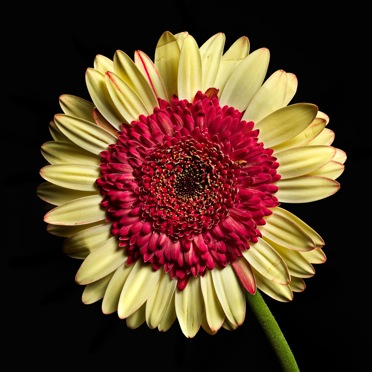
\includegraphics[scale=0.22]{img/originalFlower}}
     \subfigure[Edges]{\label{lssample}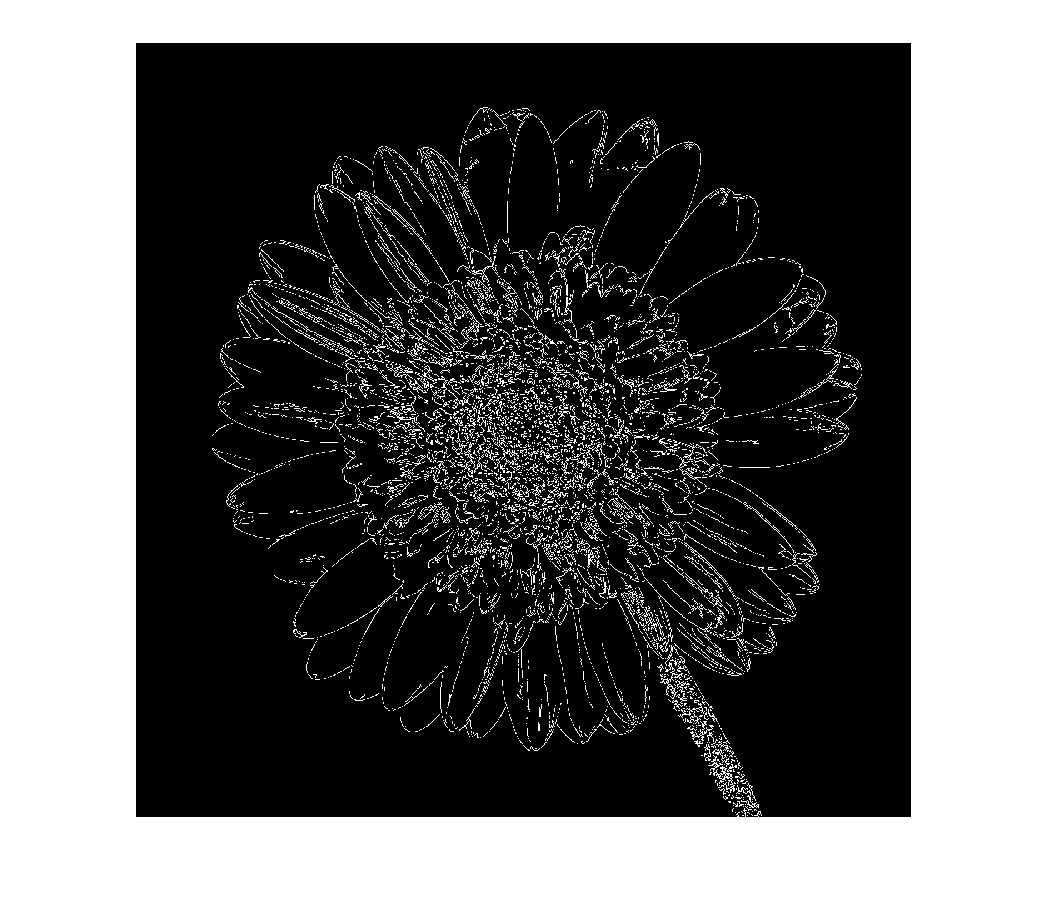
\includegraphics[scale=0.22]{img/edgesFlower}} 
     \subfigure[Corners]{\label{lssample}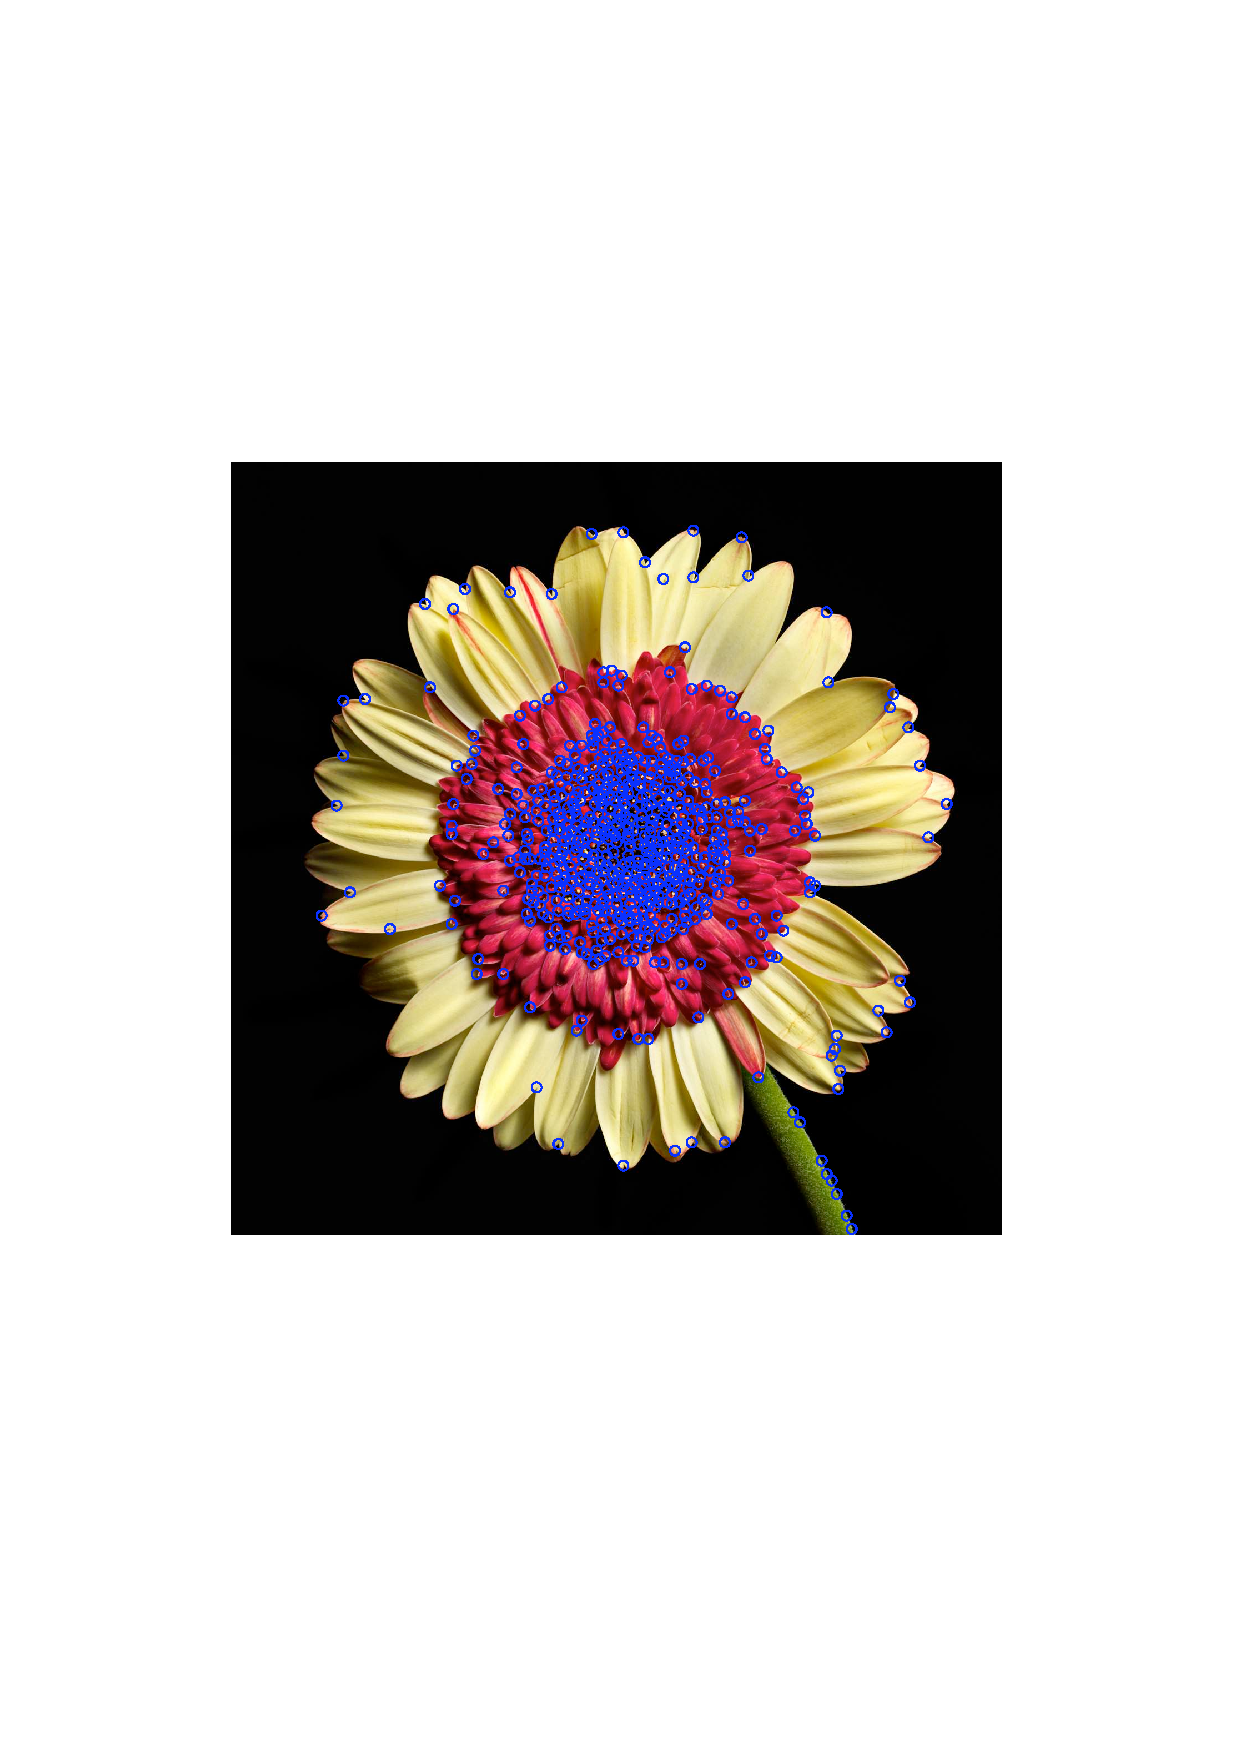
\includegraphics[scale=0.22]{img/cornersFlower}}  
     \subfigure[Hue]{\label{lssample}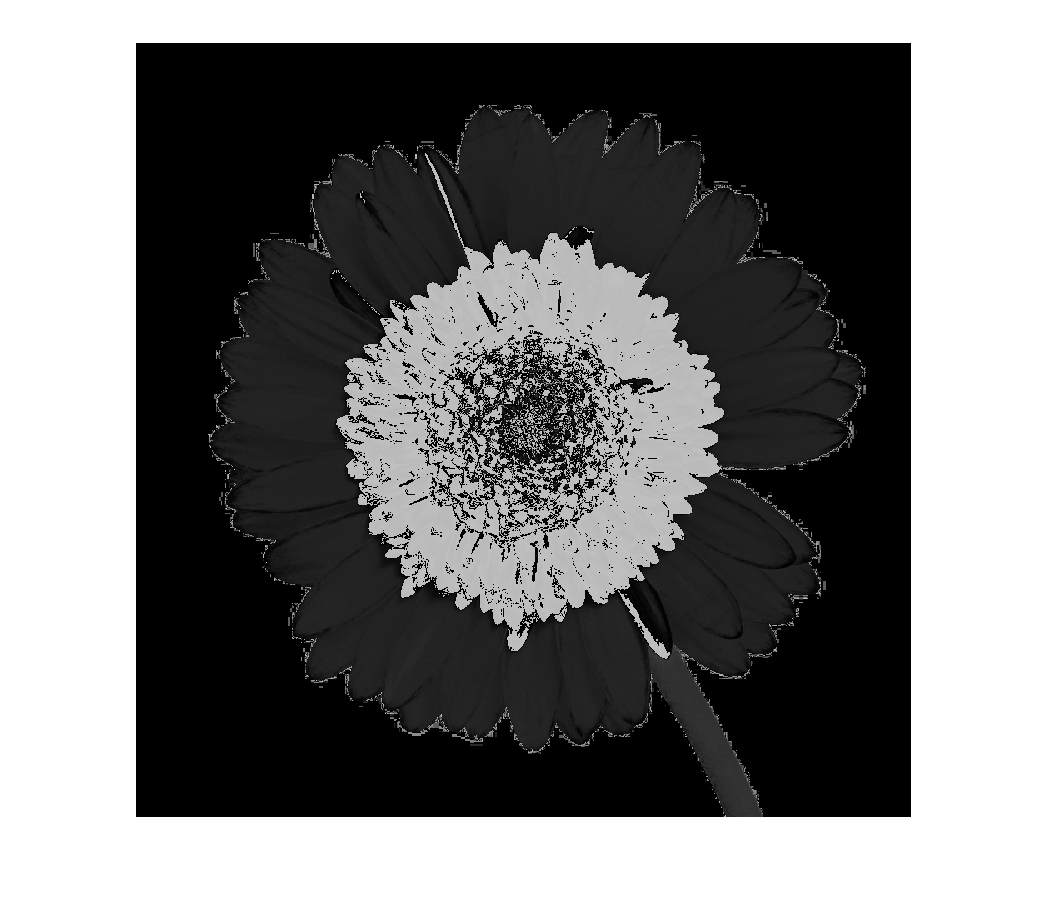
\includegraphics[scale=0.22]{img/hueFlower}}           
     \subfigure[Saturation]{\label{lssample}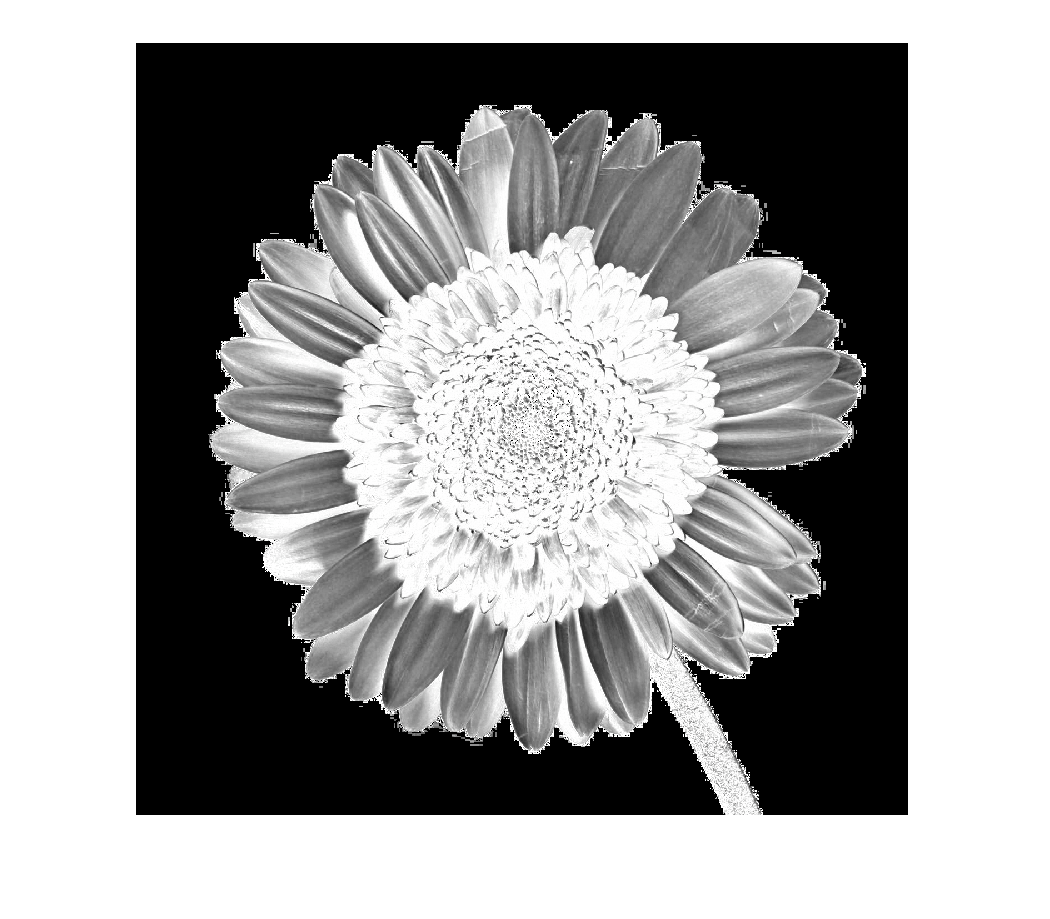
\includegraphics[scale=0.22]{img/satFlower}}           
     \subfigure[Value]{\label{lssample}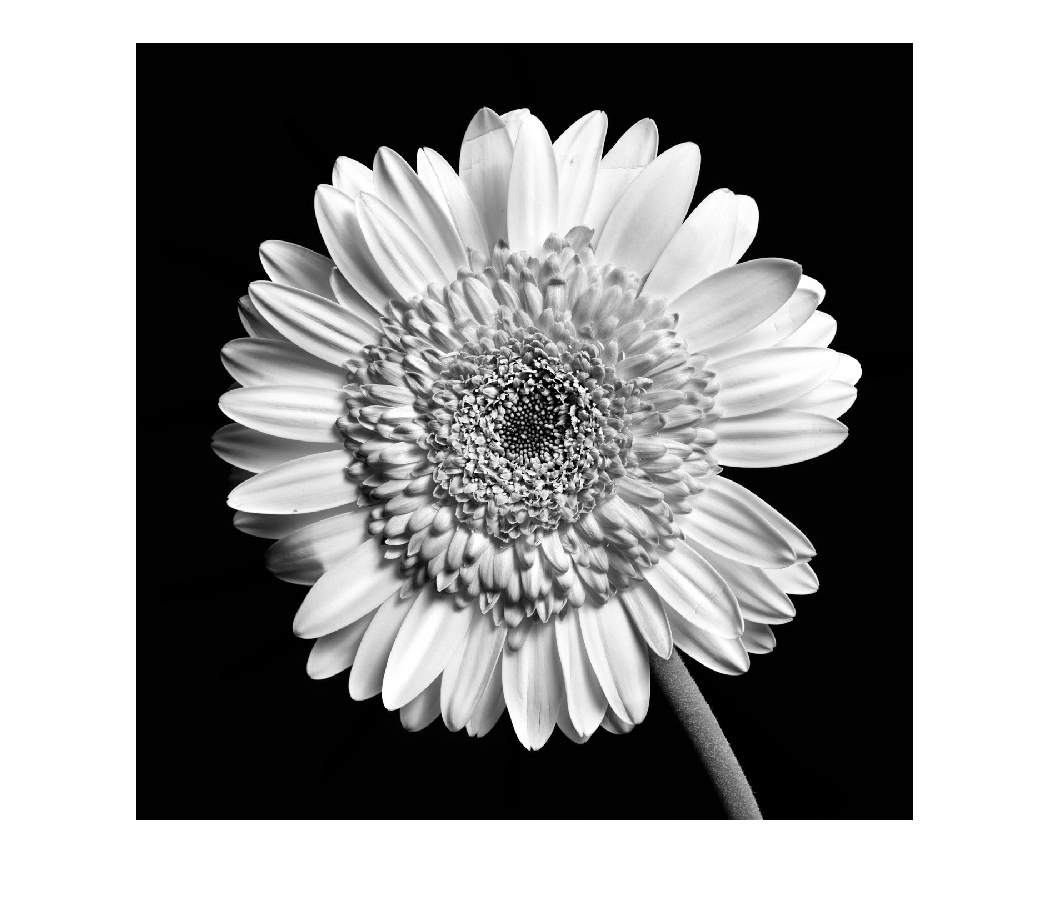
\includegraphics[scale=0.22]{img/valueFlower}}
     \subfigure[Intensity]{\label{lssample}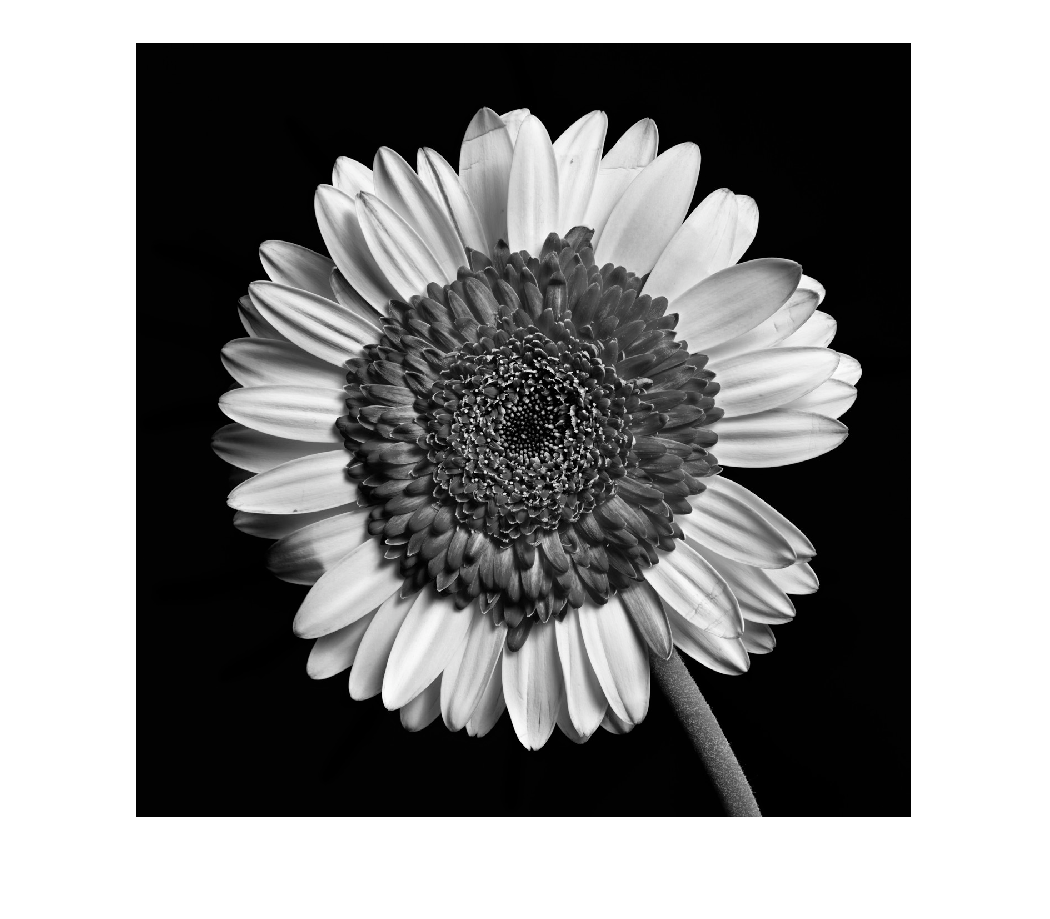
\includegraphics[scale=0.22]{img/intFlower}}                               
     \subfigure[Red]{\label{lssample}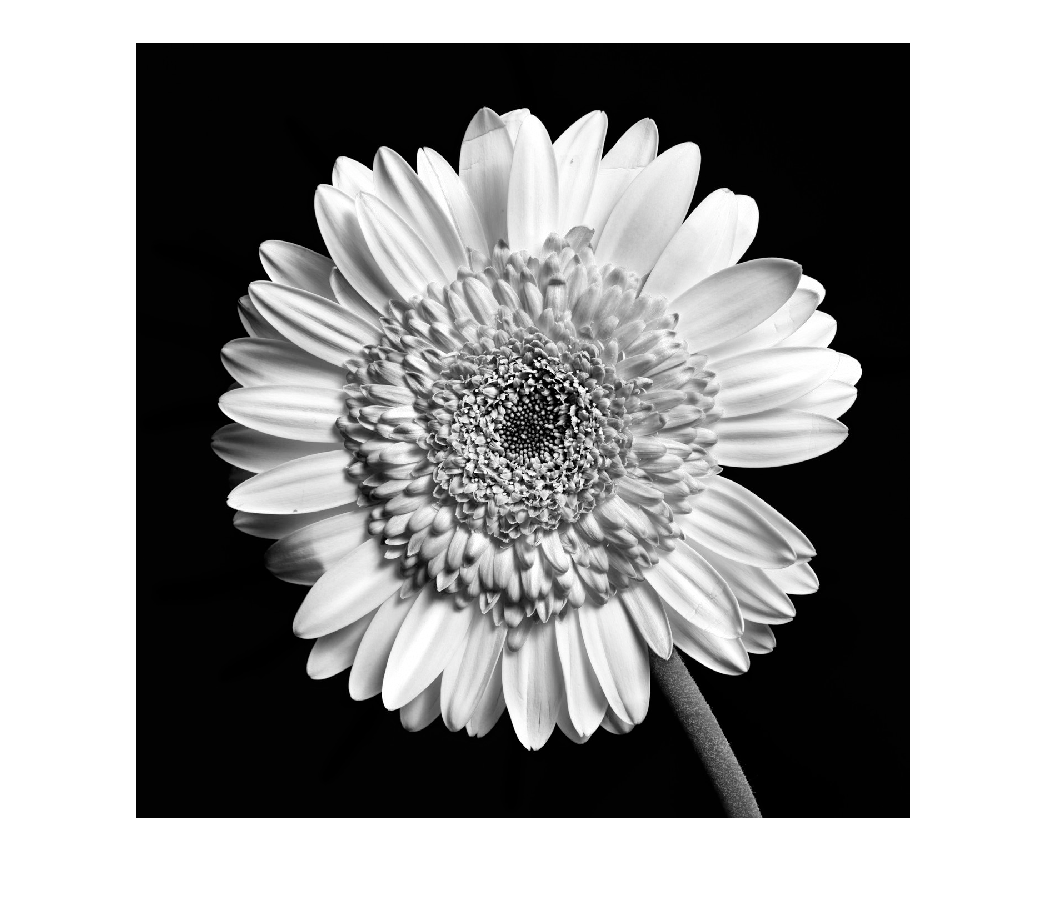
\includegraphics[scale=0.22]{img/redFlower}}
     \subfigure[Green]{\label{lssample}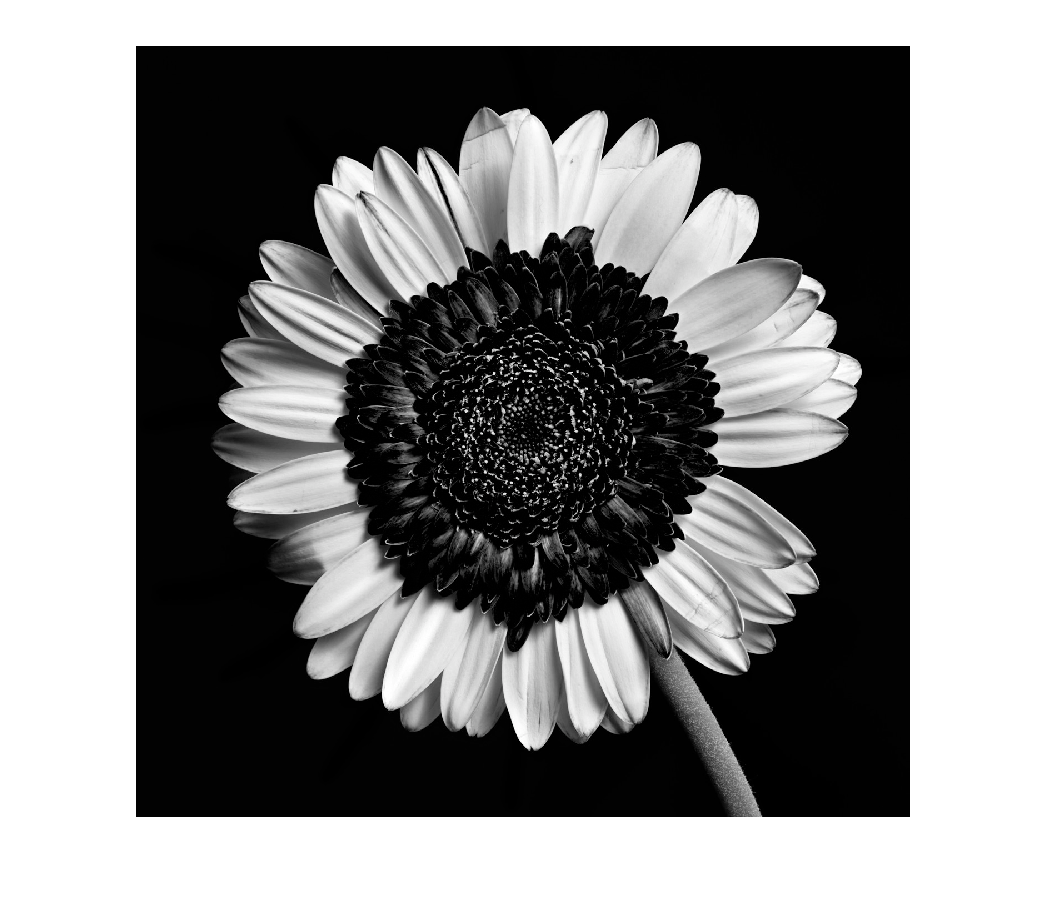
\includegraphics[scale=0.22]{img/greenFlower}}
     \subfigure[Blue]{\label{lssample}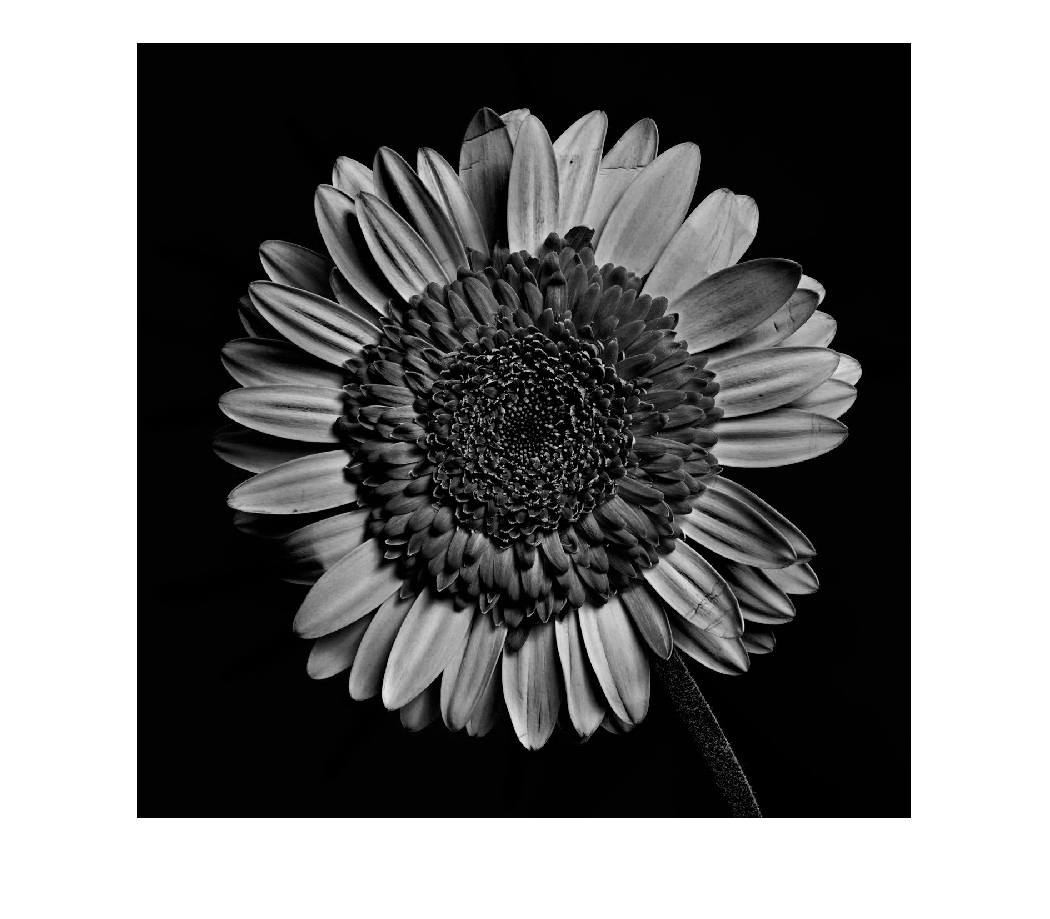
\includegraphics[scale=0.22]{img/blueFlower}}

  \end{center}
  \caption{Illustration of different statistical features}
  \label{featureImg}
\end{figure}


The features described above only contain global information about images. In order to capture localized information as well, several of the features described above are also extracted from different regions of the image. The regions of the image are obtained by dividing the image along both dimensions into NxM equal-sized regions. Since feature values will most likely vary from region region, these compositional features should provide valuable additional information about an image. 

\textbf{add reference to opencv somewhere}


%\subsubsection{Weibull, this subsubsubsection can be made normal text, but we can do that later}
%The contrast of natural image statistics has been shown to conform to Weibull-shaped probability distributions \cite{Weibull_physical}. Furthermore, when images do not adhere to this distribution, the images in question are mashups of multiple sub-images which themselves do conform to the Weibull distribution. In addition to this property of natural images, it has been proposed that the parameters for the Weibull distribution form a basis for the description of texture in images \cite{Weibull_6}. There is indeed evidence that the human visual system is capable of approximating the parameters of the Weibull distribution \cite{Weibull_brain}. Last the two most important parameters of the Weibull distribution, when it comes to natural images have a straight forward interpretation, the shape parameter the describes the resemblance to other probability distribution, from a power-law to the normal distribution, where the scale describes the how wide the distribution is. Therefore we included the maximum likelihood estimation of the Weibull-distribution for contrast of the image as used for \cite{Weibull_6} in our Feature extraction toolbox, unfortunately this seemed to give unstable results, therefore we later eliminated it. 

\subsubsection{Cognitively-inspired features \label{proposed-cognitive}}
One of the more recent trends in computer vision research in the pursuit of human-like capability is the coupling of cognition and vision into cognitive computer vision. The term cognitive computer vision has been introduced with the aim of achieving more robust, resilient, and adaptable computer vision systems by endowing them with a cognitive faculty: the ability to learn, adapt, weigh alternative solutions, and develop new strategies for analysis and interpretation.

Recent studies focused on computational models of focal visual attention. Attention has been seen to influences the processing of visual information even in the earliest areas of primate visual cortex. Even more, it has been discovered that the interaction of bottom-up sensory information and top-down attentional influences creates an integrated \textit{saliency map}, that can be defined as a topographic representation of relative stimulus strength and behavioral relevance across visual space \cite{Saliency_WWHW}. This map enables the visual system to integrate large amounts of information, even from outside the fovea, because it provides an efficient coding scheme for the potentially most relevant information in the sensory input. 
An important model based on this theory is the one provided by Itti, Koch and Niebur \cite{Itti_review}\cite{Itti_model}. The model tries to mimic the properties of primate early vision. Despite its simple architecture the model is capable of strong performance with complex natural scene.
The model work as follow: an input image is decomposed through several pre-attentive feature detection mechanisms which operate in parallel channels over the entire visual scene, and four conspicuity maps (color, orientation, intensity and skin) are created. After few different intermediate steps, the model finally combines the four conspicuity maps into a unique saliency map. 

Til now the saliency map has been used as information channel in scene understanding and object recognition. In this reasearch, image features have extracted from the map and then used in the classification and visualization task. Features that have been extracted from those maps are: \textit{Shannon entropy} of the five maps, \textit{Standard deviation} of the distribution of attention in the saliency map, \textit{Location} of the most salient points (defined as the centers of the most salient regions) and \textit{Skin intensity} of the skin map. Skin is not a default channel in the Itti's model, but it has been found out to be really interesting and useful in devianART to distinguish artists and artworks, where there is a huge presence of photographer that create nude art. 

\subsection{Describing classes with features}
An important aspect of analyzing images is to determine what makes them distinct.
In this tookit, classification is used to compare image sets and extract the image features that best separates them.
This knowledge can be used to describe the art style of an artist or even determine if there is an artist that uses an unique style.
Also classification can be extended to other category level to determine what the image features of a category are.
This section describes our approach of using a classifier to describe classes using the features described in section \ref{sec:features}. 

\subsubsection{Pre-processing}
Before classifiers can be used to find features, several pre-processing steps are required on the dataset.

Classifiers are more effective whenever the values in a dataset are in the same range(REF).
Therefore normalization is important because the features that were extracted all have different ranges of values.
For this toolkit the Min Max normalization was used in order to set all the values in the dataset in the same range.

\begin{equation}
\label{minmax}
$y$ = \frac{$x$-\min($x$)}{\max($x$)-\min($x$)}*(B-A)
\end{equation}

Formula \ref{minmax} shows the normalization equation that was used in this toolkit.
In this formula, $y$ are the translated values of a feature, $x$ are the untransformed value of a feature, $A$ is the minimum value of the new range and $B$ is the maximum value of the new range.

%Furthermore filtering on classes and features can be performed on the dataset, this is to provide flexibility in a way %that the user can do classification on just a few interesting classes or features instead of everything that is inside the %dataset.

\subsubsection{Classifiers}
The classifiers are used to determine what features are separable for a certain class.
Multiple classifiers can be chosen from to do this task.

\begin{itemize}
	\item \textbf{k-Nearest Neighbour}: It classifies images based on the closest training examples.
	This classifier uses a parameter $k$ that can be optimized. 
	The parameter indicates how many of the training examples the classifier should compare the new image with before it can classify to what class an image belongs to.
	\item \textbf{Naive Bayes}: It calculates the probability of a new image belonging to a class.
	This classifier takes every feature seperately and divide it into $N$ bins, it will then count the number of training examples for every class in all the bins and uses this to compute the posterior probability.
	$N$ is used here as a parameter that can be optimized.
	\item \textbf{Nearest Mean}: It calculates the mean value of a class and classifies new images based on how close it lays to the mean of a class.
	\item \textbf{Support Vector Machine}: It creates a model based on a set of training examples which belongs to two classes.
	The SVM tries to divide the training examples by a clear gap and then predicts the class of a new example based on which side of the gap it lays.
\end{itemize}

%The classifiers were implemented using PRTools \cite{Duin00prtoolsversion} and libSVM \cite{chang2001libsvm}, which are existing implementations of the classifiers.

\subsubsection{Feature Selection}
Whenever a person wants to find the image features that best separates two classes, that person wants to have a small list containing image features that does that.
Therefore a feature selection algorithm is needed to make sure that the classifier will only choose a few features(e.g. 1,2,3) instead of a whole list of features which does not say anything interesting.

Features were selected by using the \textit{Sequential forward feature selection} \cite{pudil1994floating}.
It selects features by first choosing the most informative feature and then iteratively add the next most informative feature to it.
Selecting the most informative feature is done using the inter-intra criterion \cite{pekalska2005pairwise}.
This criterion is computed based on the average dispersion of a class around its mean and the distance of mean to the overall average value of the dataset.
Therefore the features that are selected are the features that clusters the class while eliminating the overlap between that cluster and the other classes.

\subsubsection{Evaluation Measures}
For classification the \textit{precision} and \textit{recall} are used as evaluation measures for how well a classifier performs.
The precision is computed by measuring how many percent of the examples were correctly classified as positive as opposed to how many of all examples were classified as positive.
The recall is computed by measuring how many percent of the positive examples were indeed classified as positive.
The total performance score of the classifier can be calculated using the $F_1-measure$.
The $F_1$-measure is the weighted average of the precision and recall scores where they are both weighted as equally importance.
For our toolkit a high $F_1$-measure means that the features that were used to classify an artist are reliable features to separate the artist from the other artists in the set.

\subsubsection{Parameter Optimization}
Another important aspect of classification is to do parameter optimization. 
Optimization of parameters will lead to better classification results because the classifier is more fine tuned to the type of task that lies ahead. 
The way the optimization is presented in this toolkit is by cross-validation on the train set.
For every parameter in the classifier cross-validation is performed on the trainset to compute the F-measure score.
The average F-measure score of every fold is used as an evaluation measure to indicate how well the classifier performs.
%\end{document}